% ---------------------------------------------------------------------------
%  Section 2: Impact
% ---------------------------------------------------------------------------


\section{Impact}
\label{sec:impact}
\TOWRITE{ALL}{Describe impact}

\begin{figure}[ht]\centering
  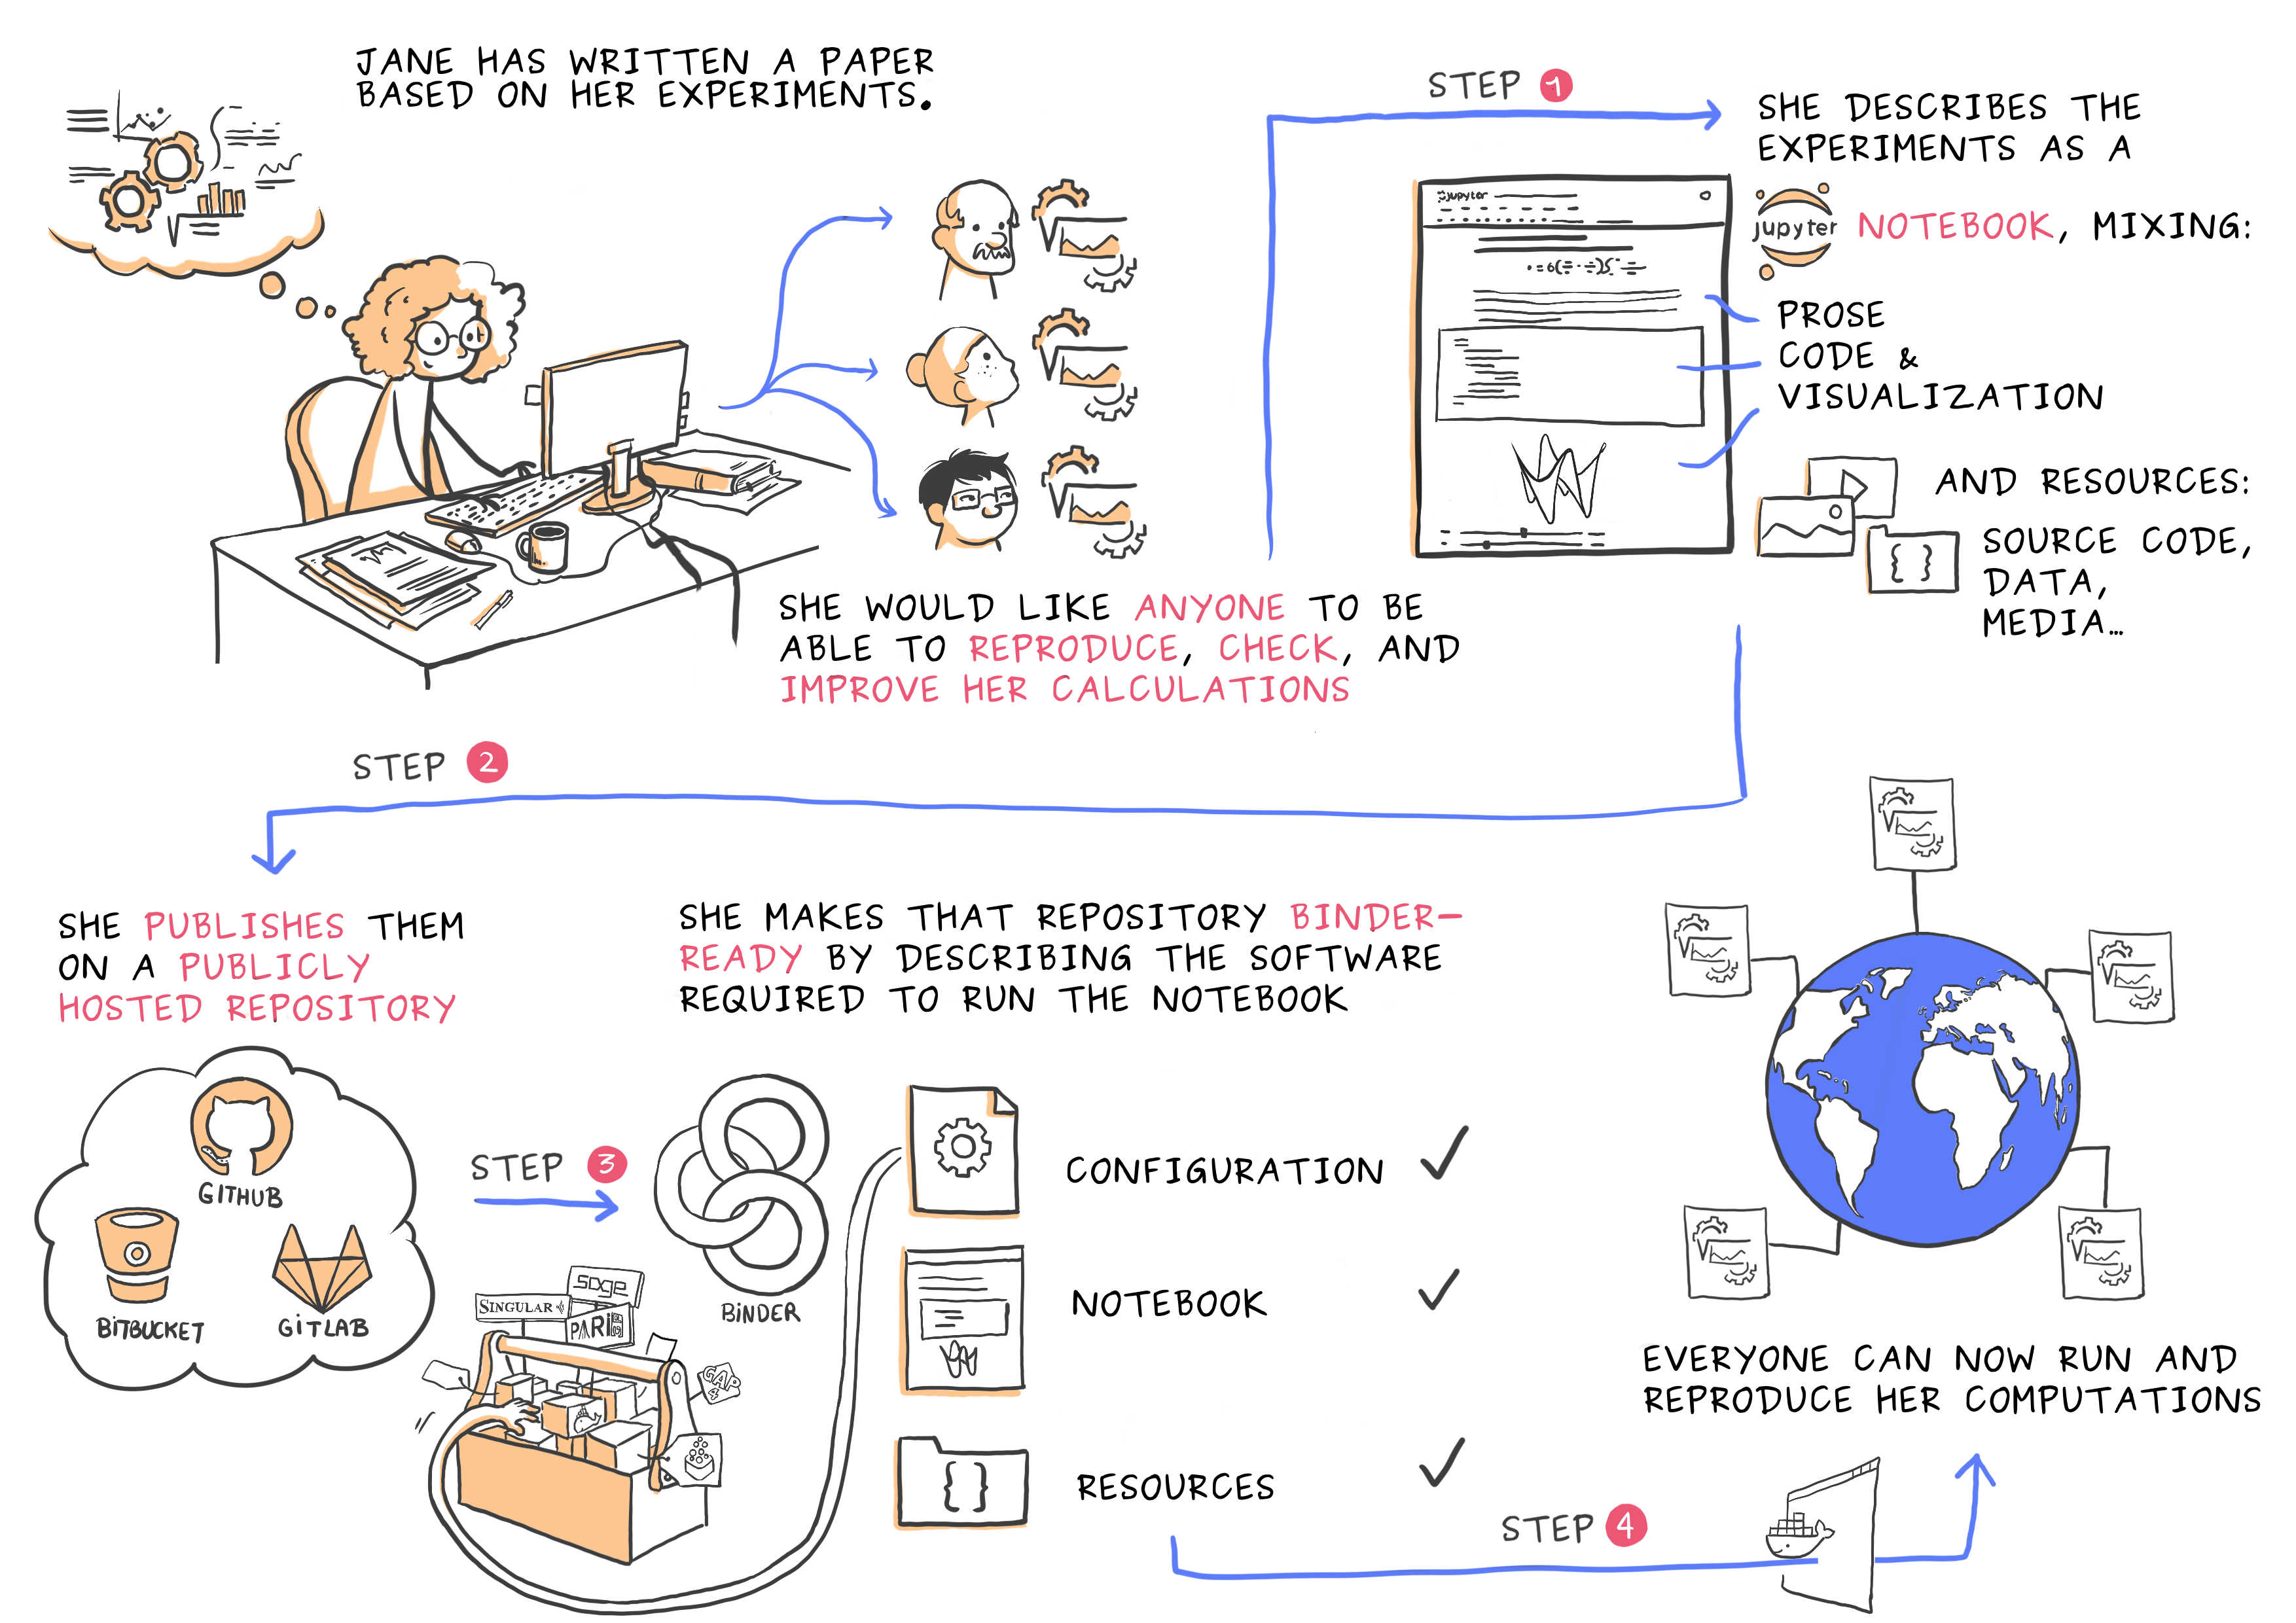
\includegraphics[width=0.9\textwidth]{use-cases-binder-logbook-solution.png}
  \caption{A typical use case for Jupyter notebooks in research.
            Image by Juliette Belin for the OpenDreamKit project, used under
            CC-BY-SA.}\label{fig:use-cases-binder}
\end{figure}

The central impact of the \TheProject project will be the wide availability of
Jupyter-based software for reproducible research on the European Open Science
Cloud. While this will initially be developed alongside applications for our
own institutions, we expect the tools we develop to be useful to a much larger
group of researchers, as data analysis and simulation are now crucial parts
of many scientific disciplines.

Jupyter-based technology will be especially valuable given the decentralised
nature of EOSC. Large-scale experiments often produce so much data that it is
impractical to transfer the data to another site for analysis.
At European XFEL, for instance, hundreds of terabytes of data may be recorded
for a single user experiment. The analysis steps thus need to run where the
data is stored, even if the scientist has returned to their home institution
far away. As the Jupyter Notebook interface runs in a web browser,
it is readily usable for remote access.

\subsection{Expected Impacts}

\eucommentary{Please be specific, and provide only information that applies
to the proposal and its objectives. Wherever possible, use quantified
indicators and targets.\\
Describe how your project will contribute to:\\
-- the expected impacts set out in the work programme, under the relevant topic
(including key performance indicators/metrics for monitoring results and impacts);\\
-- improving innovation capacity and the integration of new knowledge
(strengthening the competitiveness and growth of companies by developing
innovations meeting the needs of European and global markets; and, where
relevant, by delivering such innovations to the markets;\\
-- any other environmental and socially important impacts (if not already
covered above).\\
Describe any barriers/obstacles, and any framework conditions (such as
regulation and standards), that may determine whether and to what extent
the expected impacts will be achieved. (This should not include any risk
factors concerning implementation, as covered in section 3.2.)}

The expected impact of \TheProject with respect to the
work program is detailed in the table below.

\begin{center}
\begin{tabular}{|m{.3\textwidth}|m{.7\textwidth}|}\hline
  Expected impact & \\\hline


  Integrating co-design into research and
  development of new services to better support scientific, industrial and
  societal applications benefiting from a strong user orientation &
  The Jupyter tools have always been driven by a close connection to users; since
  the project began as IPython in 2001, many of the developers have been
  scientific researchers using the tools as they developed them. More recently,
  when Jupyter has benefitted from dedicated developer time, developers have
  remained in academic institutions, in the kind of role now referred to as
  'research software engineers', allowing day-to-day interactions with
  researchers using Jupyter in a wide range of fields.

  By supporting developers in various research institutions where the improvements
  will be used as they are developed, \TheProject will continue this invaluable
  collaboration.
  \\\hline

  Supporting the objectives of Open Science by
  improving access to content and resources, and facilitating interdisciplinary
  collaborations &
  We expect the use of notebooks in EOSC to improve access to scientific code,
  and the data which it handles. By combining code and explanation in a convenient
  digital document, notebooks encourage publishing workflows, whereas code in
  scripts or manual interactive workflows are often kept by the researchers who
  performed them. The focus on clarity and reproducibility also helps to ensure
  that data is meaningfully accessible, by preserving essential understanding to
  make sense of the raw data.

  We have already seen a good example of the Jupyter ecosystem facilitating an
  interdisciplinary collaboration: the LIGO scientific collaboration shared
  notebooks detailing the data processing steps which led to the discovery of
  gravitational waves, using the Binder service to allow anyone to re-compute
  the published plots. Scientists with no background in gravitational waves
  studied these notebooks and improved the signal processing.
  In this proposal, we want to provide this ability to a wider audience through
  EOSC, including for disciplines which rely on processing much larger volumes of
  data. \TOWRITE{ALL}{Citation for the LIGO story?}
  \\\hline

  Fostering the innovation potential by opening up
  the EOSC ecosystem of e-infrastructure service providers to new innovative
  actors &
  Jupyter is a collection of open source software built around openly documented
  protocols and formats, along with familiar technologies such as HTML and the
  Python programming language. It's easy for third parties to create new
  tools and services using and integrating Jupyter, as evidenced by the thriving
  ecosystem of tools already in development, both by commercial and non-commercial
  actors. To highlight just one example, the first version of the popular Binder
  service was developed by a group at the Howard Hughes Medical Institute,
  working independently of the core Jupyter maintainers, but building on the
  powerful capabilities provided by Jupyter.
  \\\hline

\end{tabular}
\end{center}

